\documentclass[11pt]{article}
\usepackage[textwidth=18.0cm, textheight=23.0cm, top=2.0cm]{geometry}
\usepackage{pst-all}
\usepackage{amssymb}
\usepackage{tikz}
\usepackage{underscore}\begin{document}
\pagestyle{empty}


ClassName: \underline{\textbf{Class_05.2bp-21}}
\par
BinSize: \underline{\textbf{100 × 100}}
\par
ReduceSize: \underline{\textbf{100 × 100}}
\par
TypeNum: \underline{\textbf{60}}
\par
Num: \underline{\textbf{60}}
\par
OutS: \underline{\textbf{170000}}
\par
InS: \underline{\textbf{144220}}
\par
Rate: \underline{\textbf{0.848}}
\par
UB: \underline{\textbf{17}}
\par
LB0: \underline{\textbf{17}}
\par
LB: \underline{\textbf{17}}
\par
LBWithCut: \underline{\textbf{17}}
\par
NodeCut: \underline{\textbf{0}}
\par
ExtendedNodeCnt: \underline{\textbf{1}}
\par
GenNodeCnt: \underline{\textbf{1}}
\par
PrimalNode: \underline{\textbf{0}}
\par
ColumnCount: \underline{\textbf{17}}
\par
TotalCutCount: \underline{\textbf{0}}
\par
RootCutCount: \underline{\textbf{0}}
\par
LPSolverCnt: \underline{\textbf{1}}
\par
PricingSolverCnt: \underline{\textbf{0}}
\par
BranchAndBoundNum: \underline{\textbf{1}}
\par
isOpt: \underline{\textbf{true}}
\par
TimeOnInitSolution: \underline{\textbf{600.000 s}}
\par
TimeOnPrimal: \underline{\textbf{0.000 s}}
\par
TimeOnPricing: \underline{\textbf{0.000 s}}
\par
TimeOnRmp: \underline{\textbf{0.063 s}}
\par
TotalTime: \underline{\textbf{600.344 s}}
\par
\newpage


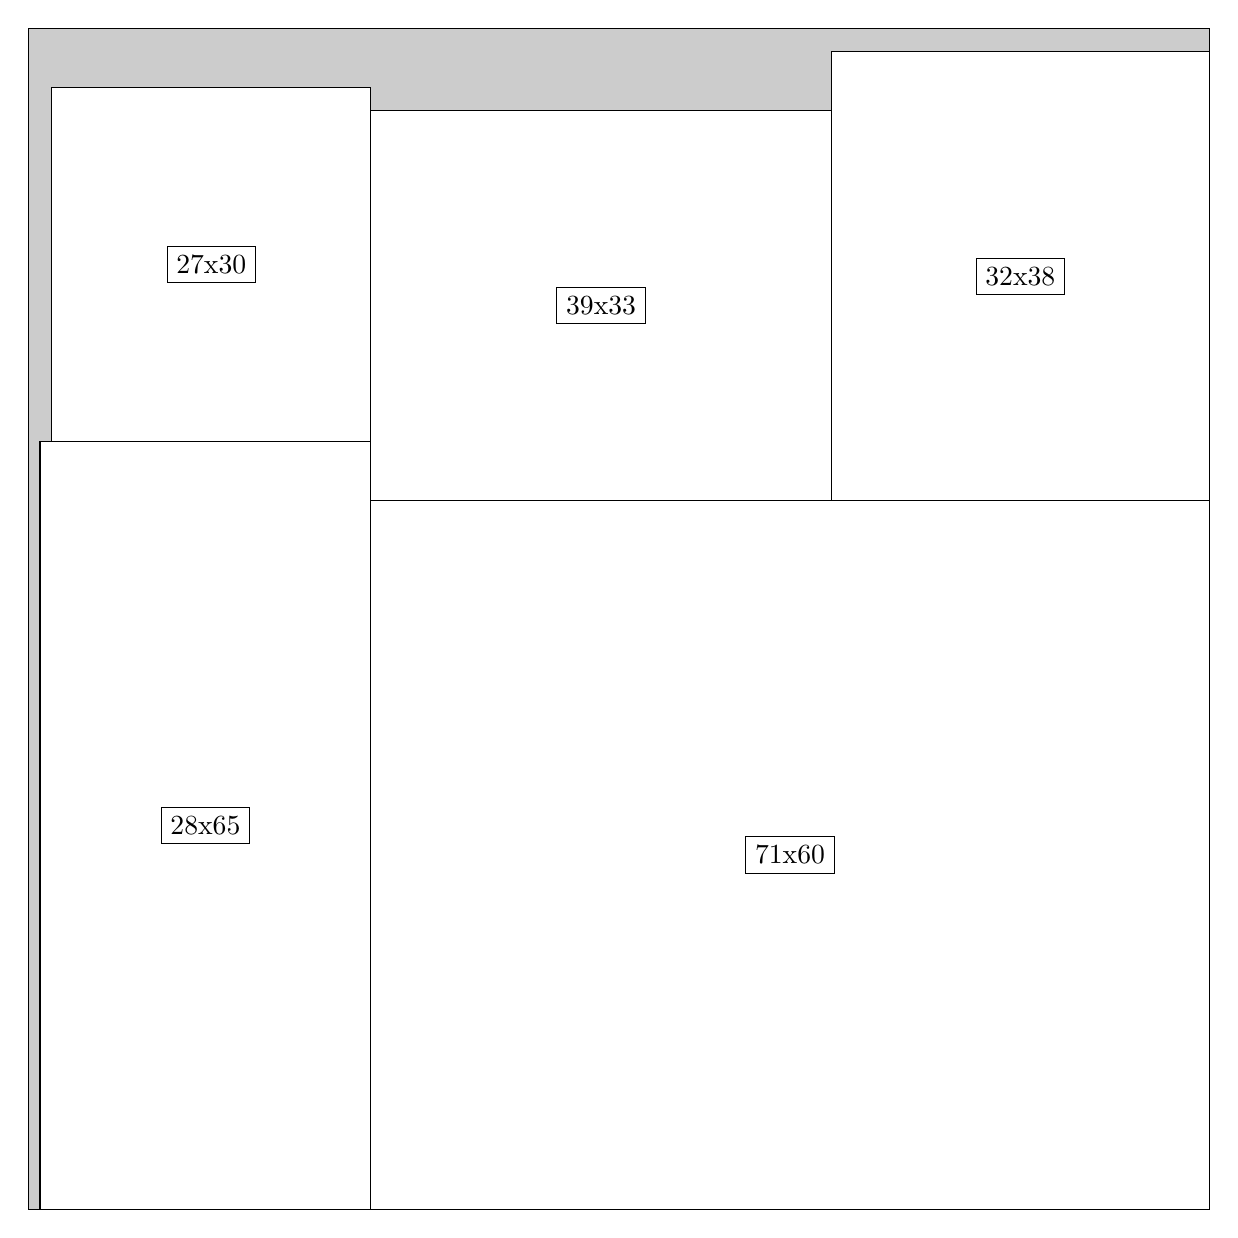
\begin{tikzpicture}[shorten >=1pt,scale=1.0,every node/.style={scale=1.0},->]
\tikzstyle{vertex}=[circle,fill=black!25,minimum size=14pt,inner sep=0pt]
\filldraw[fill=gray!40!white, draw=black] (0,0) rectangle (15.0,15.0);
\foreach \name/\x/\y/\w/\h in {71x60/4.35/0.0/10.65/9.0,32x38/10.2/9.0/4.8/5.7,39x33/4.35/9.0/5.85/4.95,28x65/0.15/0.0/4.2/9.75,27x30/0.3/9.75/4.05/4.5}
\filldraw[fill=white!40!white, draw=black] (\x,\y) rectangle node[draw] (\name) {\name} ++(\w,\h);
\end{tikzpicture}


w =71 , h =60 , x =29 , y =0 , v =4260
\par
w =32 , h =38 , x =68 , y =60 , v =1216
\par
w =39 , h =33 , x =29 , y =60 , v =1287
\par
w =28 , h =65 , x =1 , y =0 , v =1820
\par
w =27 , h =30 , x =2 , y =65 , v =810
\par
\newpage


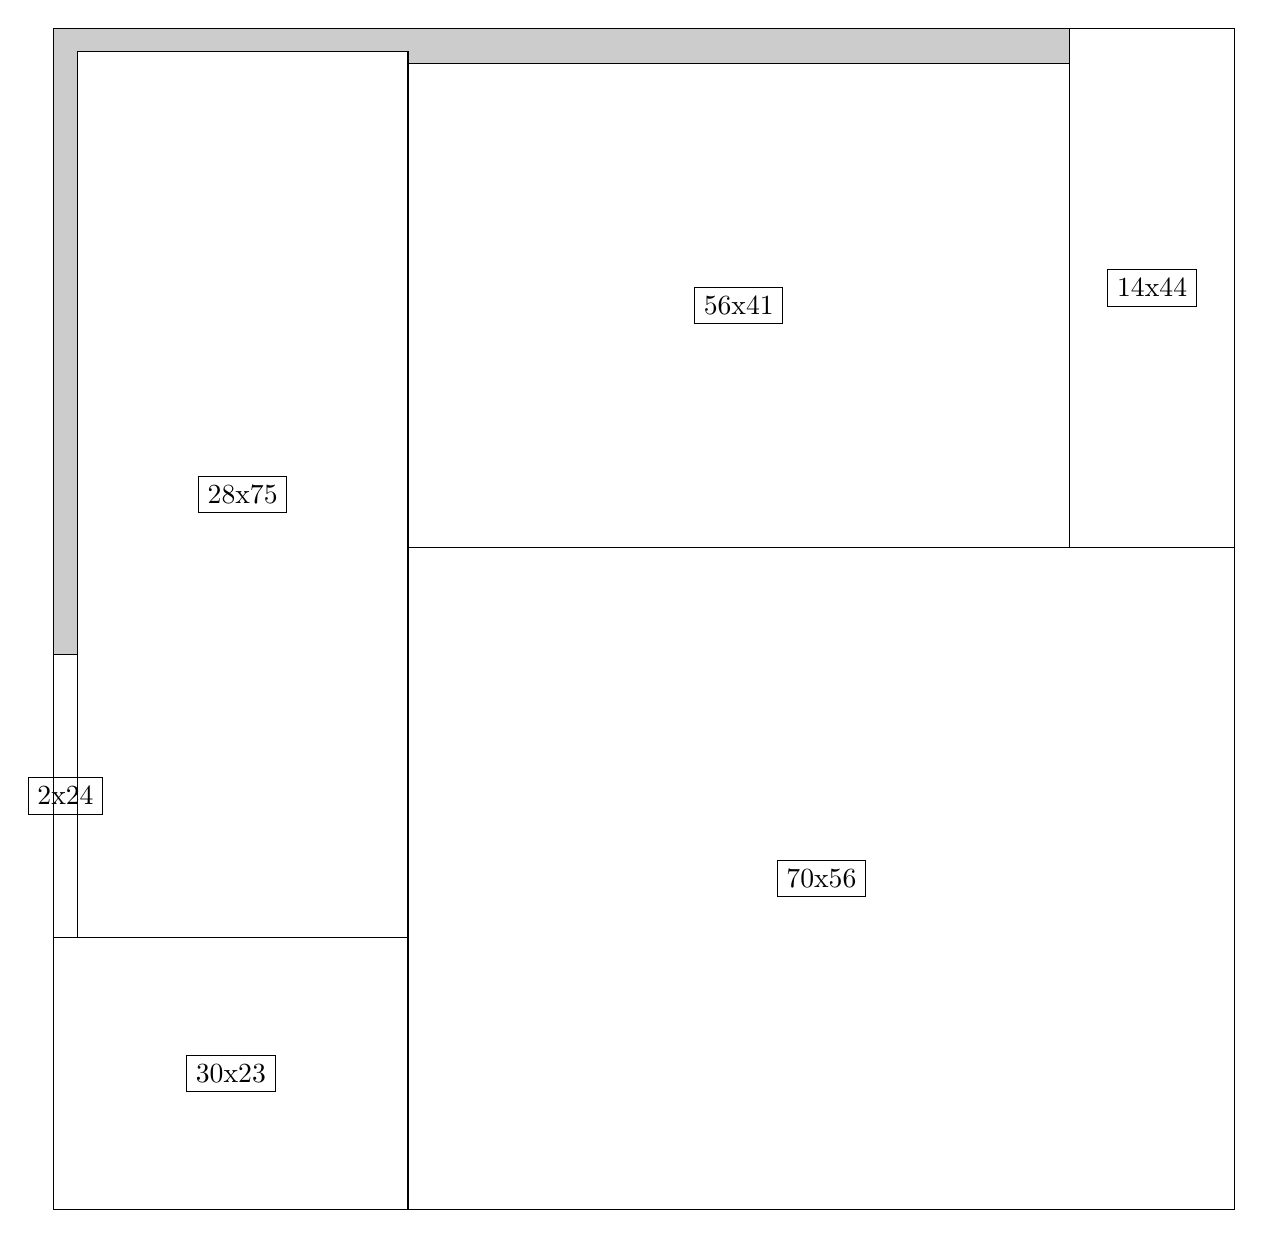
\begin{tikzpicture}[shorten >=1pt,scale=1.0,every node/.style={scale=1.0},->]
\tikzstyle{vertex}=[circle,fill=black!25,minimum size=14pt,inner sep=0pt]
\filldraw[fill=gray!40!white, draw=black] (0,0) rectangle (15.0,15.0);
\foreach \name/\x/\y/\w/\h in {70x56/4.5/0.0/10.5/8.4,14x44/12.9/8.4/2.1/6.6,56x41/4.5/8.4/8.4/6.1499999999999995,30x23/0.0/0.0/4.5/3.4499999999999997,28x75/0.3/3.4499999999999997/4.2/11.25,2x24/0.0/3.4499999999999997/0.3/3.5999999999999996}
\filldraw[fill=white!40!white, draw=black] (\x,\y) rectangle node[draw] (\name) {\name} ++(\w,\h);
\end{tikzpicture}


w =70 , h =56 , x =30 , y =0 , v =3920
\par
w =14 , h =44 , x =86 , y =56 , v =616
\par
w =56 , h =41 , x =30 , y =56 , v =2296
\par
w =30 , h =23 , x =0 , y =0 , v =690
\par
w =28 , h =75 , x =2 , y =23 , v =2100
\par
w =2 , h =24 , x =0 , y =23 , v =48
\par
\newpage


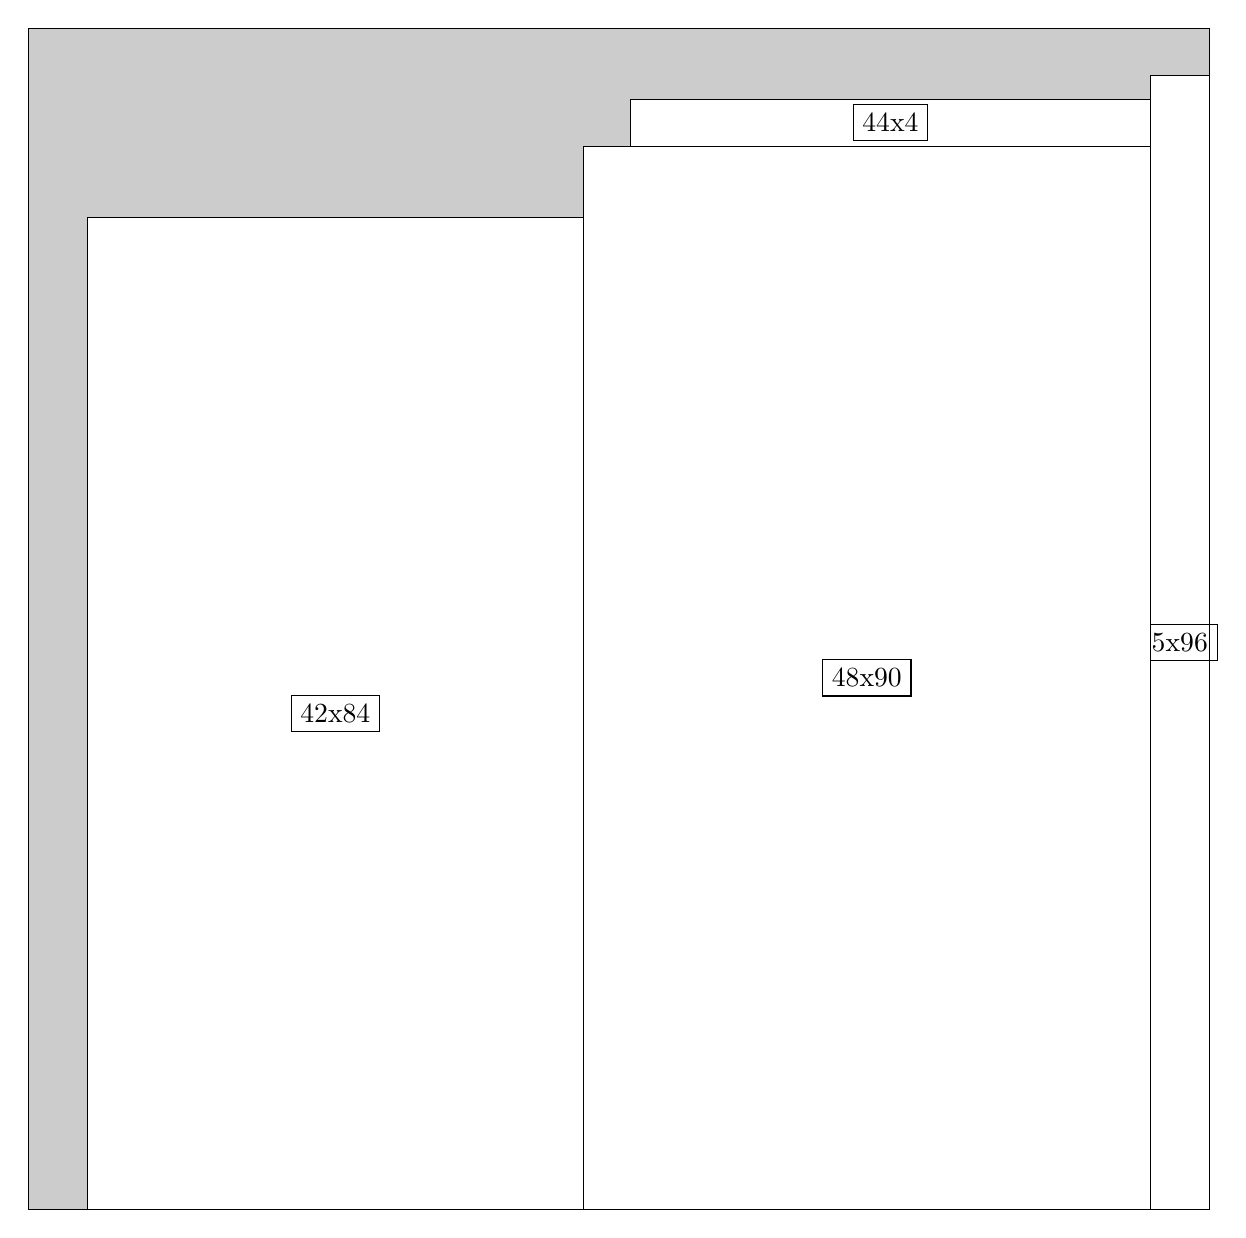
\begin{tikzpicture}[shorten >=1pt,scale=1.0,every node/.style={scale=1.0},->]
\tikzstyle{vertex}=[circle,fill=black!25,minimum size=14pt,inner sep=0pt]
\filldraw[fill=gray!40!white, draw=black] (0,0) rectangle (15.0,15.0);
\foreach \name/\x/\y/\w/\h in {5x96/14.25/0.0/0.75/14.399999999999999,48x90/7.05/0.0/7.199999999999999/13.5,44x4/7.6499999999999995/13.5/6.6/0.6,42x84/0.75/0.0/6.3/12.6}
\filldraw[fill=white!40!white, draw=black] (\x,\y) rectangle node[draw] (\name) {\name} ++(\w,\h);
\end{tikzpicture}


w =5 , h =96 , x =95 , y =0 , v =480
\par
w =48 , h =90 , x =47 , y =0 , v =4320
\par
w =44 , h =4 , x =51 , y =90 , v =176
\par
w =42 , h =84 , x =5 , y =0 , v =3528
\par
\newpage


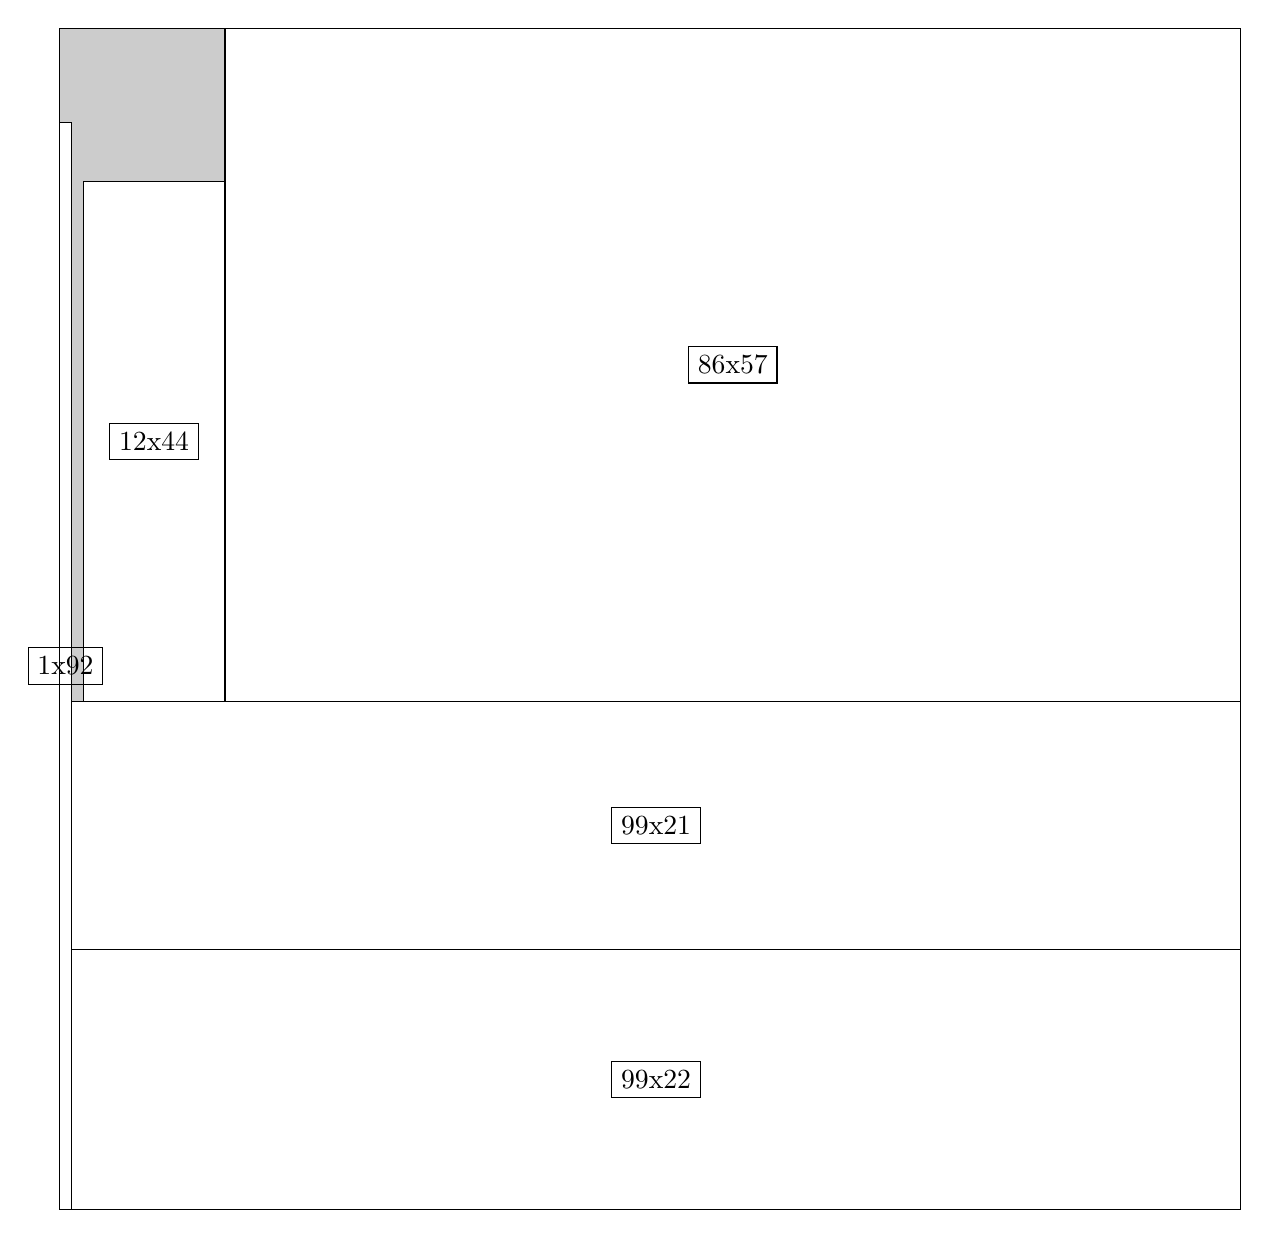
\begin{tikzpicture}[shorten >=1pt,scale=1.0,every node/.style={scale=1.0},->]
\tikzstyle{vertex}=[circle,fill=black!25,minimum size=14pt,inner sep=0pt]
\filldraw[fill=gray!40!white, draw=black] (0,0) rectangle (15.0,15.0);
\foreach \name/\x/\y/\w/\h in {99x22/0.15/0.0/14.85/3.3,99x21/0.15/3.3/14.85/3.15,86x57/2.1/6.45/12.9/8.549999999999999,12x44/0.3/6.45/1.7999999999999998/6.6,1x92/0.0/0.0/0.15/13.799999999999999}
\filldraw[fill=white!40!white, draw=black] (\x,\y) rectangle node[draw] (\name) {\name} ++(\w,\h);
\end{tikzpicture}


w =99 , h =22 , x =1 , y =0 , v =2178
\par
w =99 , h =21 , x =1 , y =22 , v =2079
\par
w =86 , h =57 , x =14 , y =43 , v =4902
\par
w =12 , h =44 , x =2 , y =43 , v =528
\par
w =1 , h =92 , x =0 , y =0 , v =92
\par
\newpage


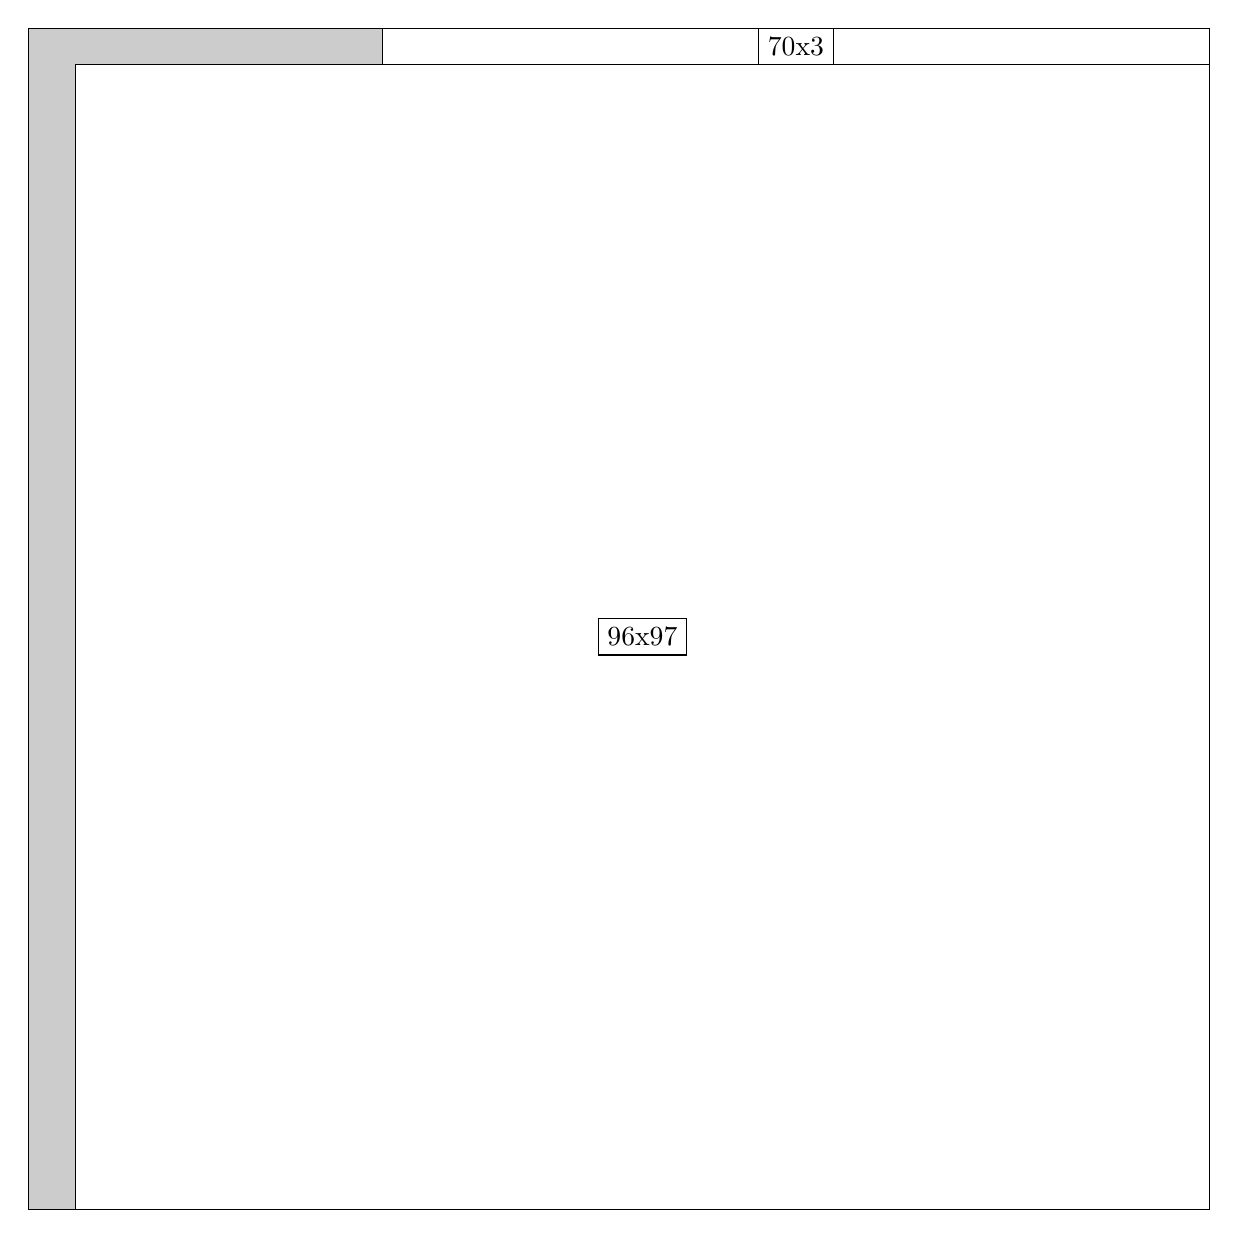
\begin{tikzpicture}[shorten >=1pt,scale=1.0,every node/.style={scale=1.0},->]
\tikzstyle{vertex}=[circle,fill=black!25,minimum size=14pt,inner sep=0pt]
\filldraw[fill=gray!40!white, draw=black] (0,0) rectangle (15.0,15.0);
\foreach \name/\x/\y/\w/\h in {96x97/0.6/0.0/14.399999999999999/14.549999999999999,70x3/4.5/14.549999999999999/10.5/0.44999999999999996}
\filldraw[fill=white!40!white, draw=black] (\x,\y) rectangle node[draw] (\name) {\name} ++(\w,\h);
\end{tikzpicture}


w =96 , h =97 , x =4 , y =0 , v =9312
\par
w =70 , h =3 , x =30 , y =97 , v =210
\par
\newpage


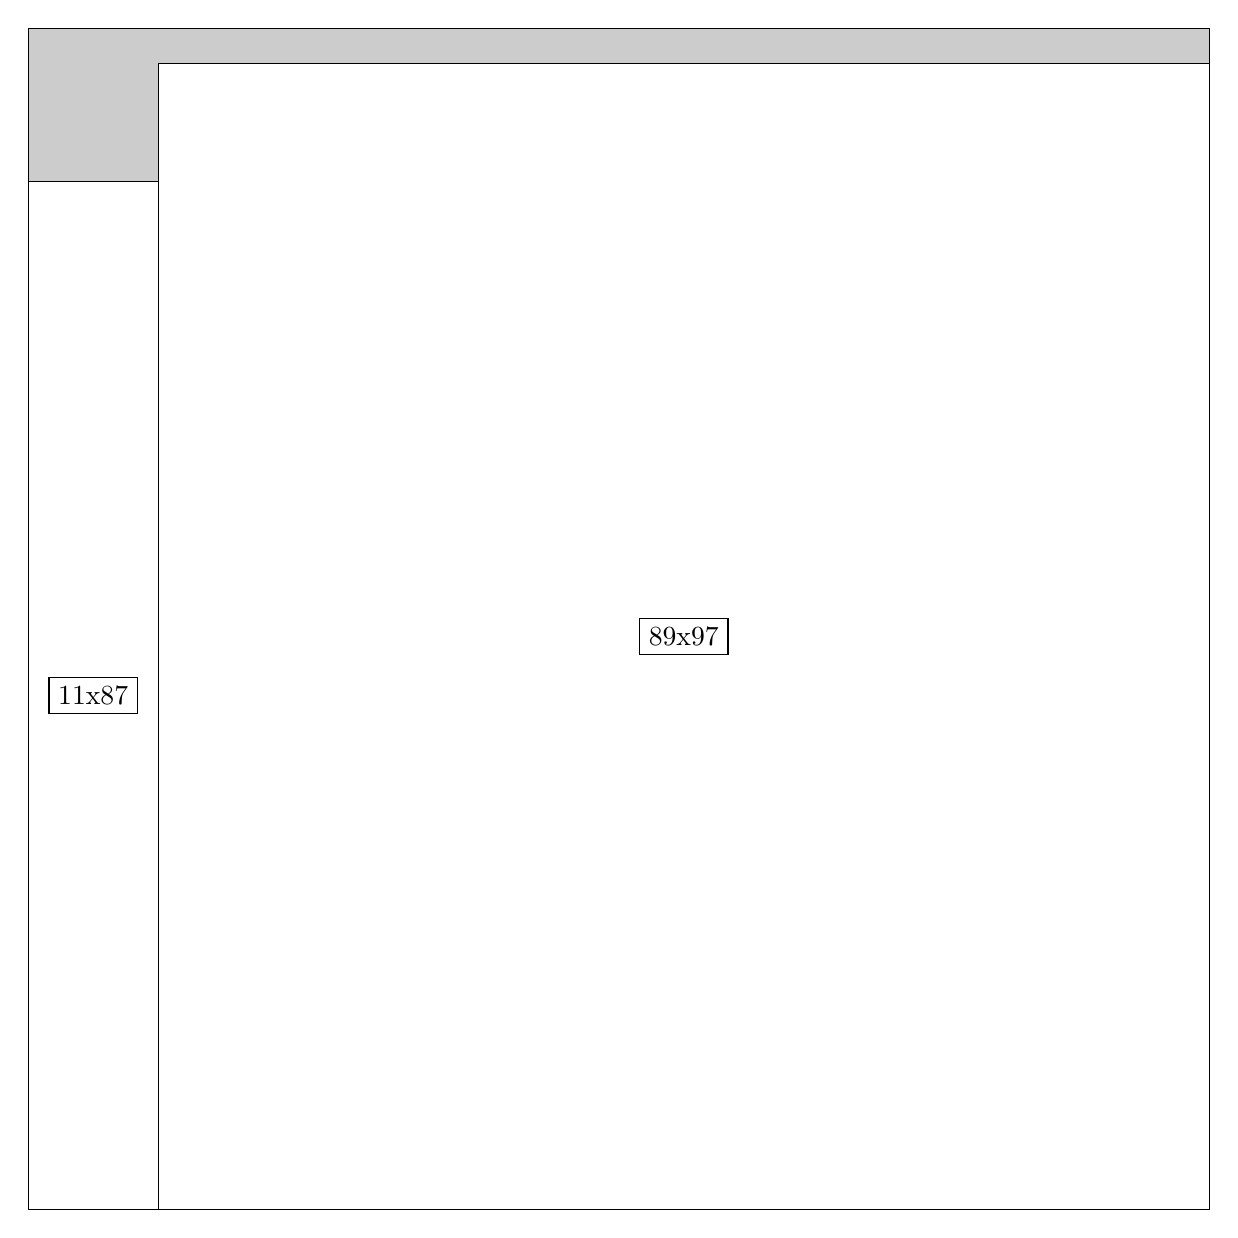
\begin{tikzpicture}[shorten >=1pt,scale=1.0,every node/.style={scale=1.0},->]
\tikzstyle{vertex}=[circle,fill=black!25,minimum size=14pt,inner sep=0pt]
\filldraw[fill=gray!40!white, draw=black] (0,0) rectangle (15.0,15.0);
\foreach \name/\x/\y/\w/\h in {89x97/1.65/0.0/13.35/14.549999999999999,11x87/0.0/0.0/1.65/13.049999999999999}
\filldraw[fill=white!40!white, draw=black] (\x,\y) rectangle node[draw] (\name) {\name} ++(\w,\h);
\end{tikzpicture}


w =89 , h =97 , x =11 , y =0 , v =8633
\par
w =11 , h =87 , x =0 , y =0 , v =957
\par
\newpage



\begin{tikzpicture}[shorten >=1pt,scale=1.0,every node/.style={scale=1.0},->]
\tikzstyle{vertex}=[circle,fill=black!25,minimum size=14pt,inner sep=0pt]
\filldraw[fill=gray!40!white, draw=black] (0,0) rectangle (15.0,15.0);
\foreach \name/\x/\y/\w/\h in {95x94/0.75/0.0/14.25/14.1}
\filldraw[fill=white!40!white, draw=black] (\x,\y) rectangle node[draw] (\name) {\name} ++(\w,\h);
\end{tikzpicture}


w =95 , h =94 , x =5 , y =0 , v =8930
\par
\newpage


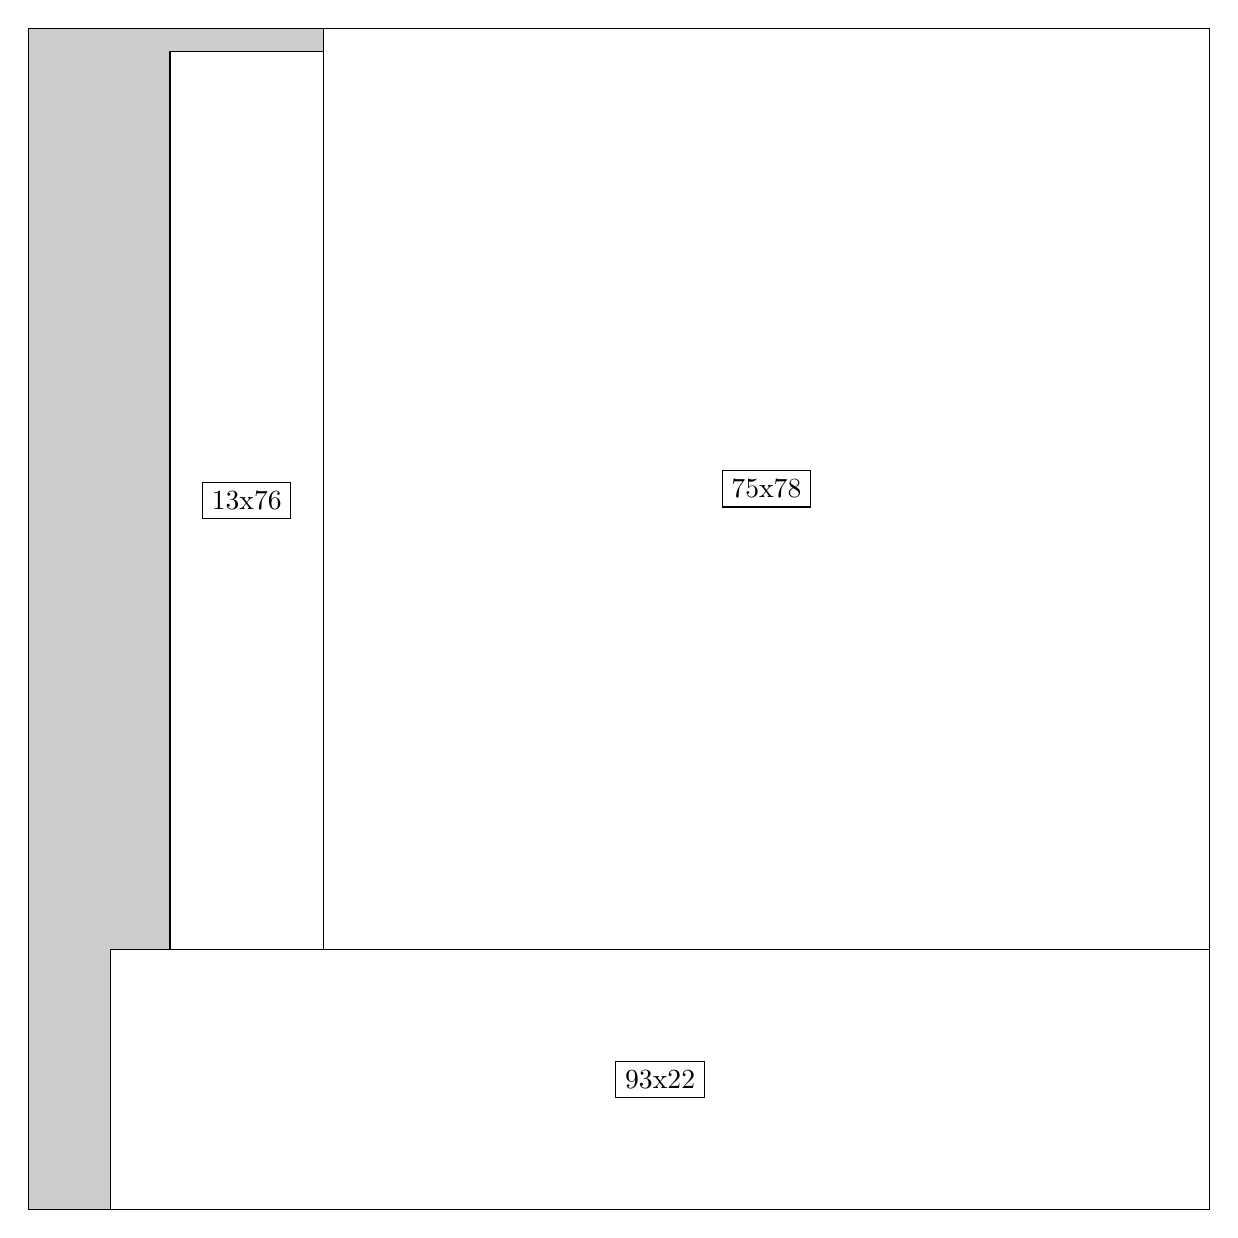
\begin{tikzpicture}[shorten >=1pt,scale=1.0,every node/.style={scale=1.0},->]
\tikzstyle{vertex}=[circle,fill=black!25,minimum size=14pt,inner sep=0pt]
\filldraw[fill=gray!40!white, draw=black] (0,0) rectangle (15.0,15.0);
\foreach \name/\x/\y/\w/\h in {93x22/1.05/0.0/13.95/3.3,75x78/3.75/3.3/11.25/11.7,13x76/1.7999999999999998/3.3/1.95/11.4}
\filldraw[fill=white!40!white, draw=black] (\x,\y) rectangle node[draw] (\name) {\name} ++(\w,\h);
\end{tikzpicture}


w =93 , h =22 , x =7 , y =0 , v =2046
\par
w =75 , h =78 , x =25 , y =22 , v =5850
\par
w =13 , h =76 , x =12 , y =22 , v =988
\par
\newpage


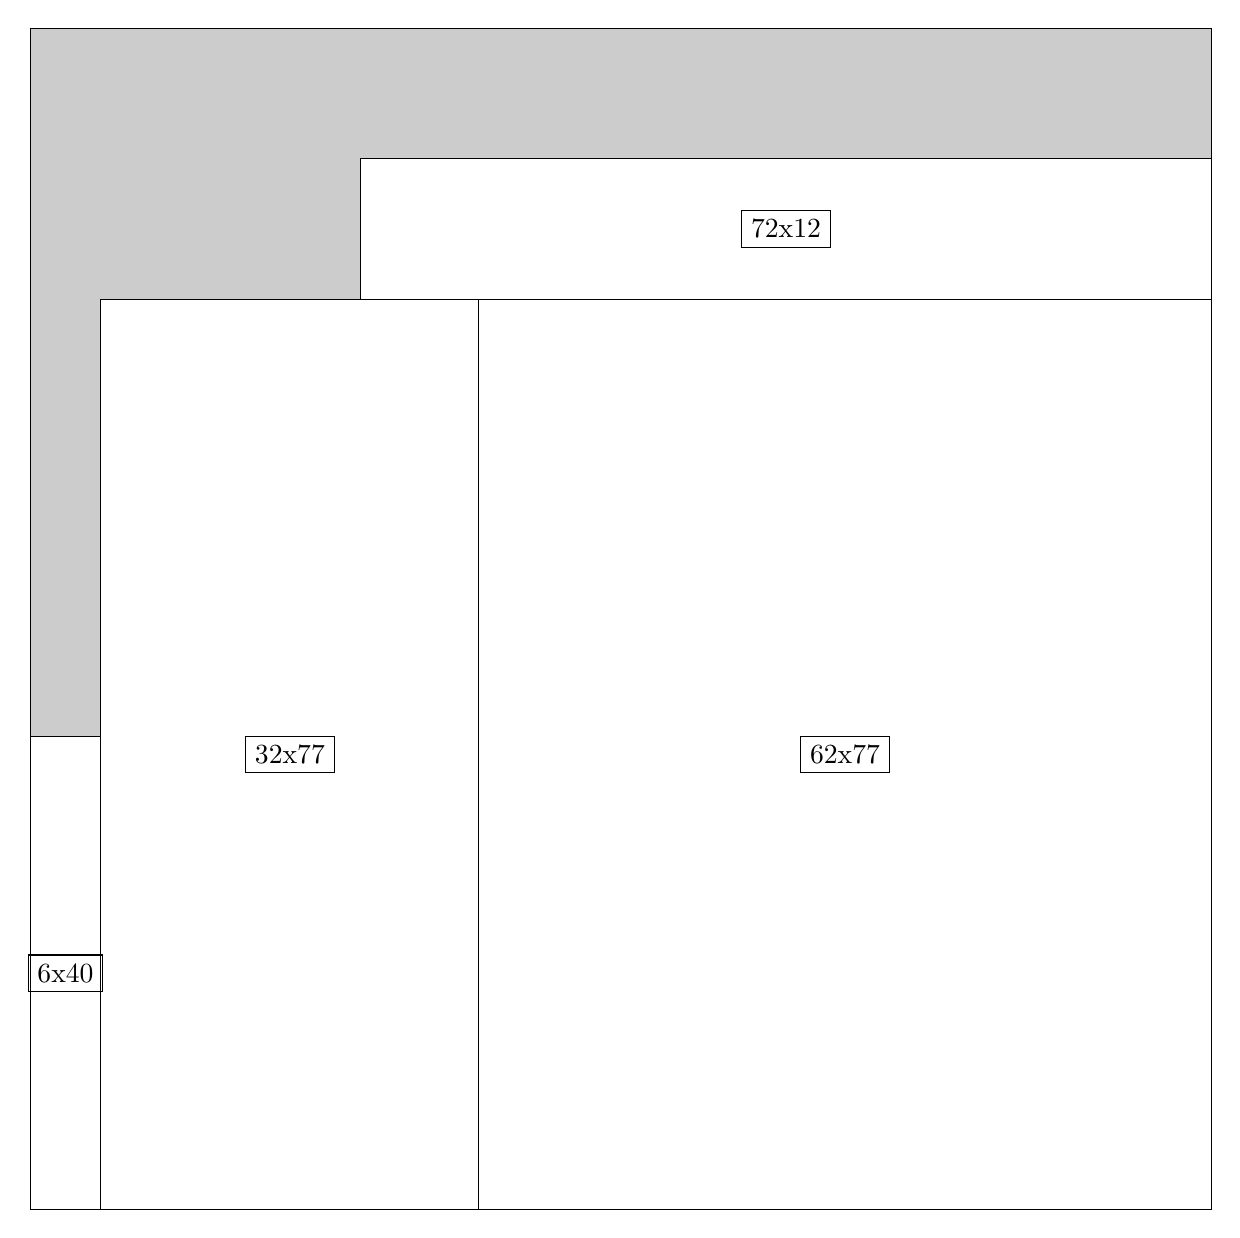
\begin{tikzpicture}[shorten >=1pt,scale=1.0,every node/.style={scale=1.0},->]
\tikzstyle{vertex}=[circle,fill=black!25,minimum size=14pt,inner sep=0pt]
\filldraw[fill=gray!40!white, draw=black] (0,0) rectangle (15.0,15.0);
\foreach \name/\x/\y/\w/\h in {62x77/5.7/0.0/9.299999999999999/11.549999999999999,32x77/0.8999999999999999/0.0/4.8/11.549999999999999,6x40/0.0/0.0/0.8999999999999999/6.0,72x12/4.2/11.549999999999999/10.799999999999999/1.7999999999999998}
\filldraw[fill=white!40!white, draw=black] (\x,\y) rectangle node[draw] (\name) {\name} ++(\w,\h);
\end{tikzpicture}


w =62 , h =77 , x =38 , y =0 , v =4774
\par
w =32 , h =77 , x =6 , y =0 , v =2464
\par
w =6 , h =40 , x =0 , y =0 , v =240
\par
w =72 , h =12 , x =28 , y =77 , v =864
\par
\newpage


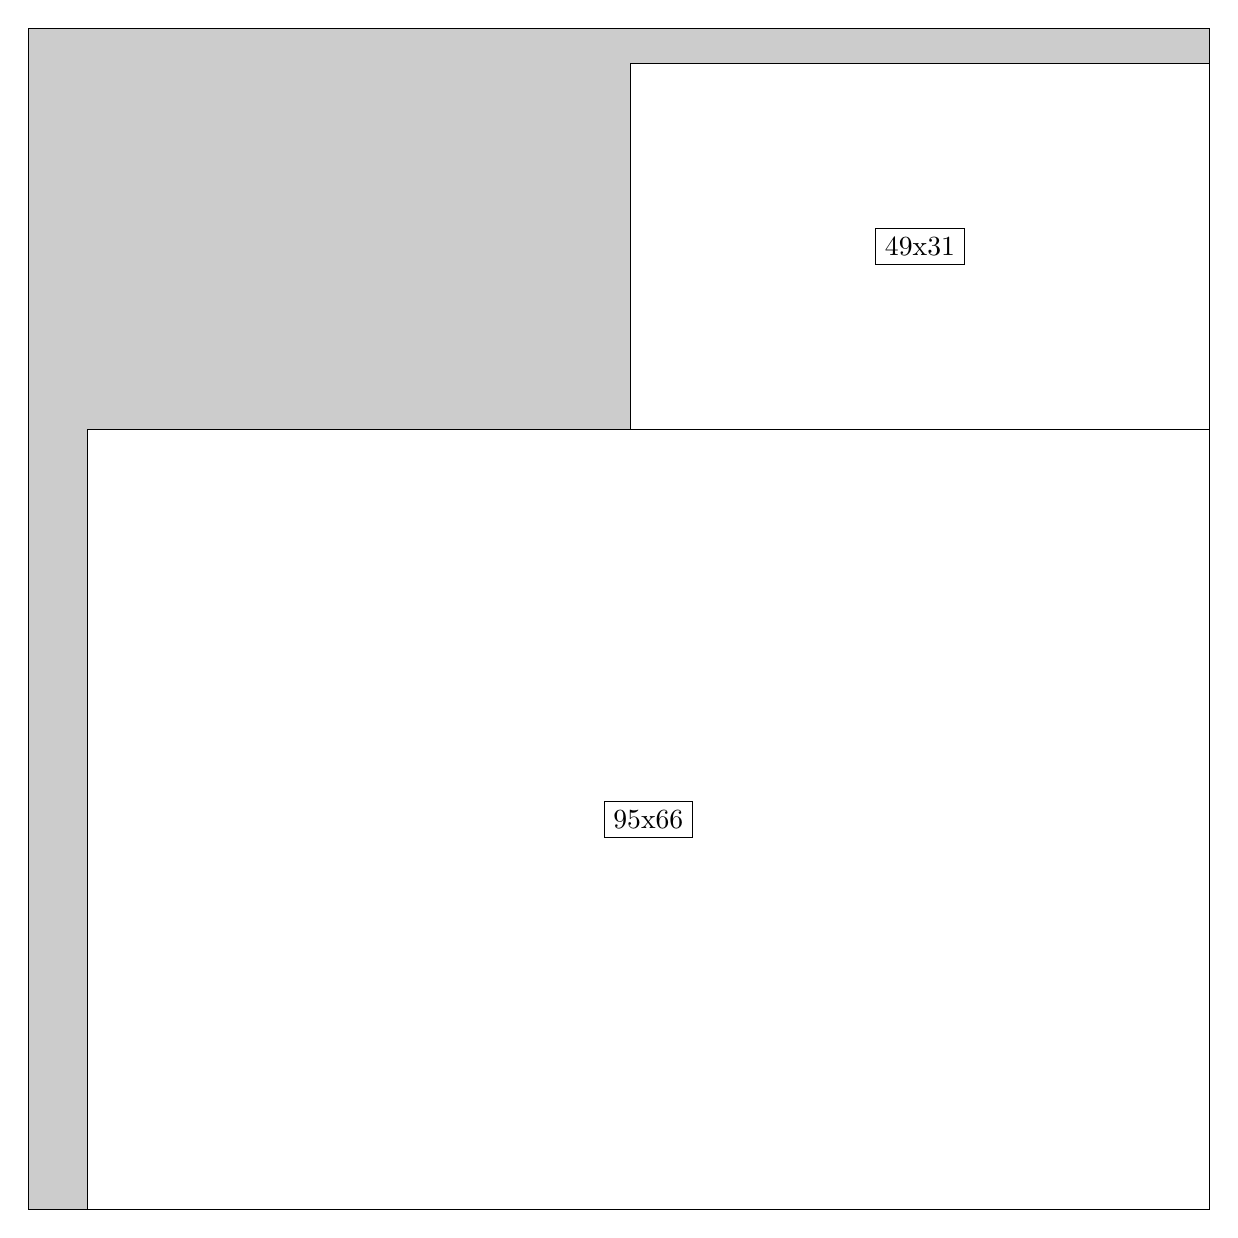
\begin{tikzpicture}[shorten >=1pt,scale=1.0,every node/.style={scale=1.0},->]
\tikzstyle{vertex}=[circle,fill=black!25,minimum size=14pt,inner sep=0pt]
\filldraw[fill=gray!40!white, draw=black] (0,0) rectangle (15.0,15.0);
\foreach \name/\x/\y/\w/\h in {95x66/0.75/0.0/14.25/9.9,49x31/7.6499999999999995/9.9/7.35/4.6499999999999995}
\filldraw[fill=white!40!white, draw=black] (\x,\y) rectangle node[draw] (\name) {\name} ++(\w,\h);
\end{tikzpicture}


w =95 , h =66 , x =5 , y =0 , v =6270
\par
w =49 , h =31 , x =51 , y =66 , v =1519
\par
\newpage


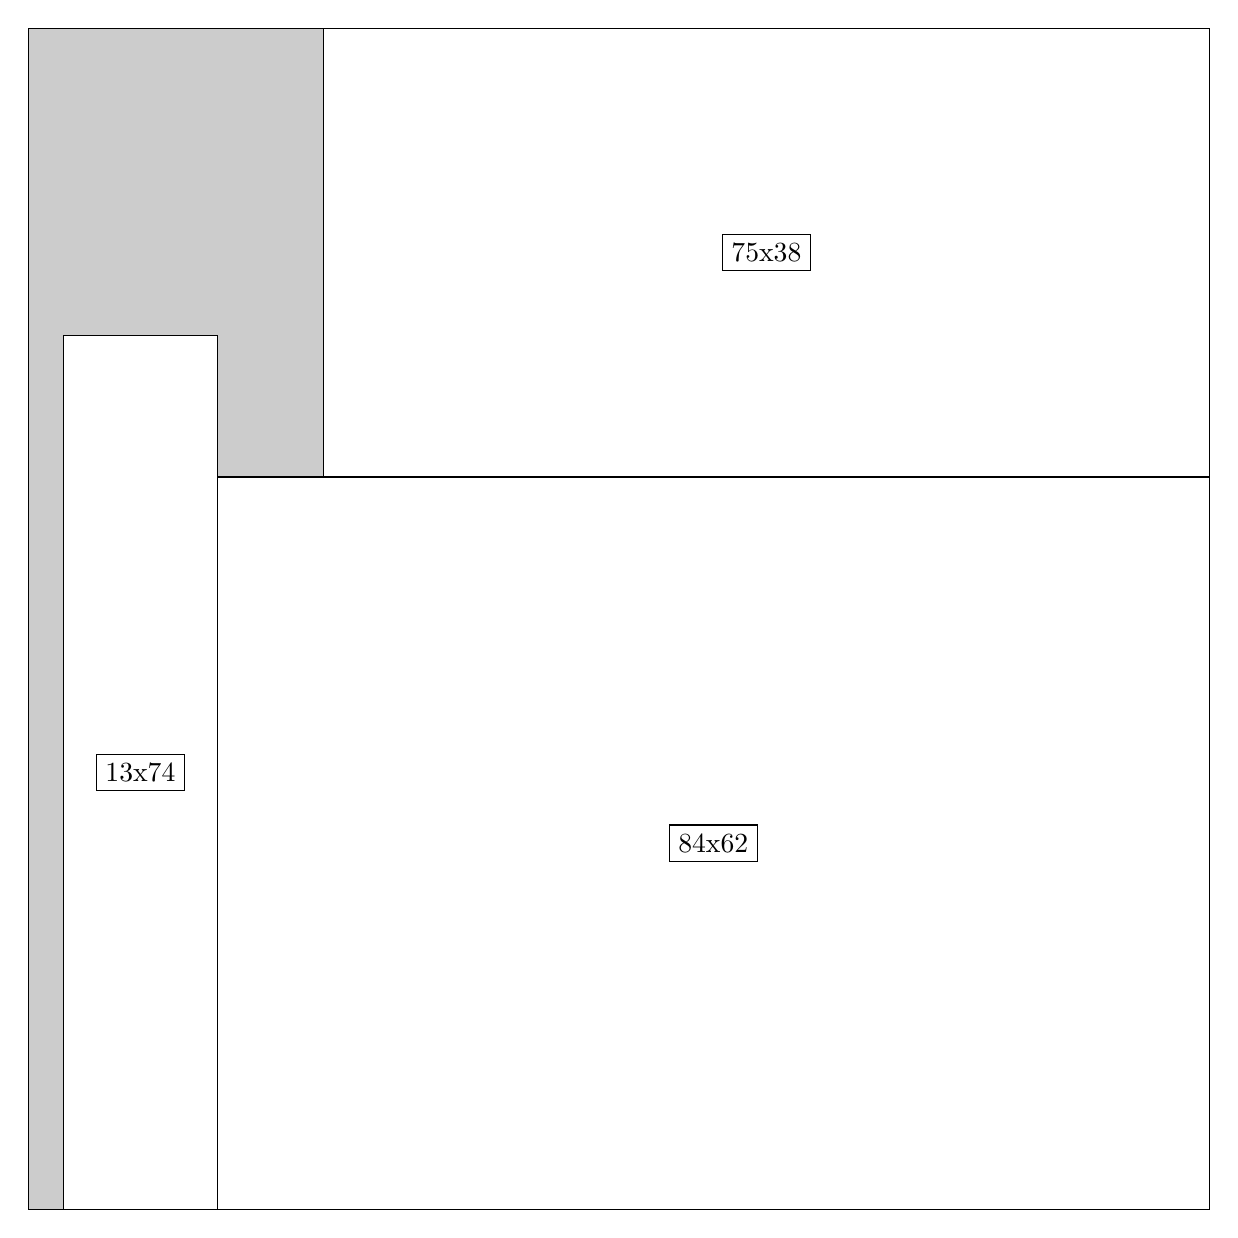
\begin{tikzpicture}[shorten >=1pt,scale=1.0,every node/.style={scale=1.0},->]
\tikzstyle{vertex}=[circle,fill=black!25,minimum size=14pt,inner sep=0pt]
\filldraw[fill=gray!40!white, draw=black] (0,0) rectangle (15.0,15.0);
\foreach \name/\x/\y/\w/\h in {84x62/2.4/0.0/12.6/9.299999999999999,75x38/3.75/9.299999999999999/11.25/5.7,13x74/0.44999999999999996/0.0/1.95/11.1}
\filldraw[fill=white!40!white, draw=black] (\x,\y) rectangle node[draw] (\name) {\name} ++(\w,\h);
\end{tikzpicture}


w =84 , h =62 , x =16 , y =0 , v =5208
\par
w =75 , h =38 , x =25 , y =62 , v =2850
\par
w =13 , h =74 , x =3 , y =0 , v =962
\par
\newpage


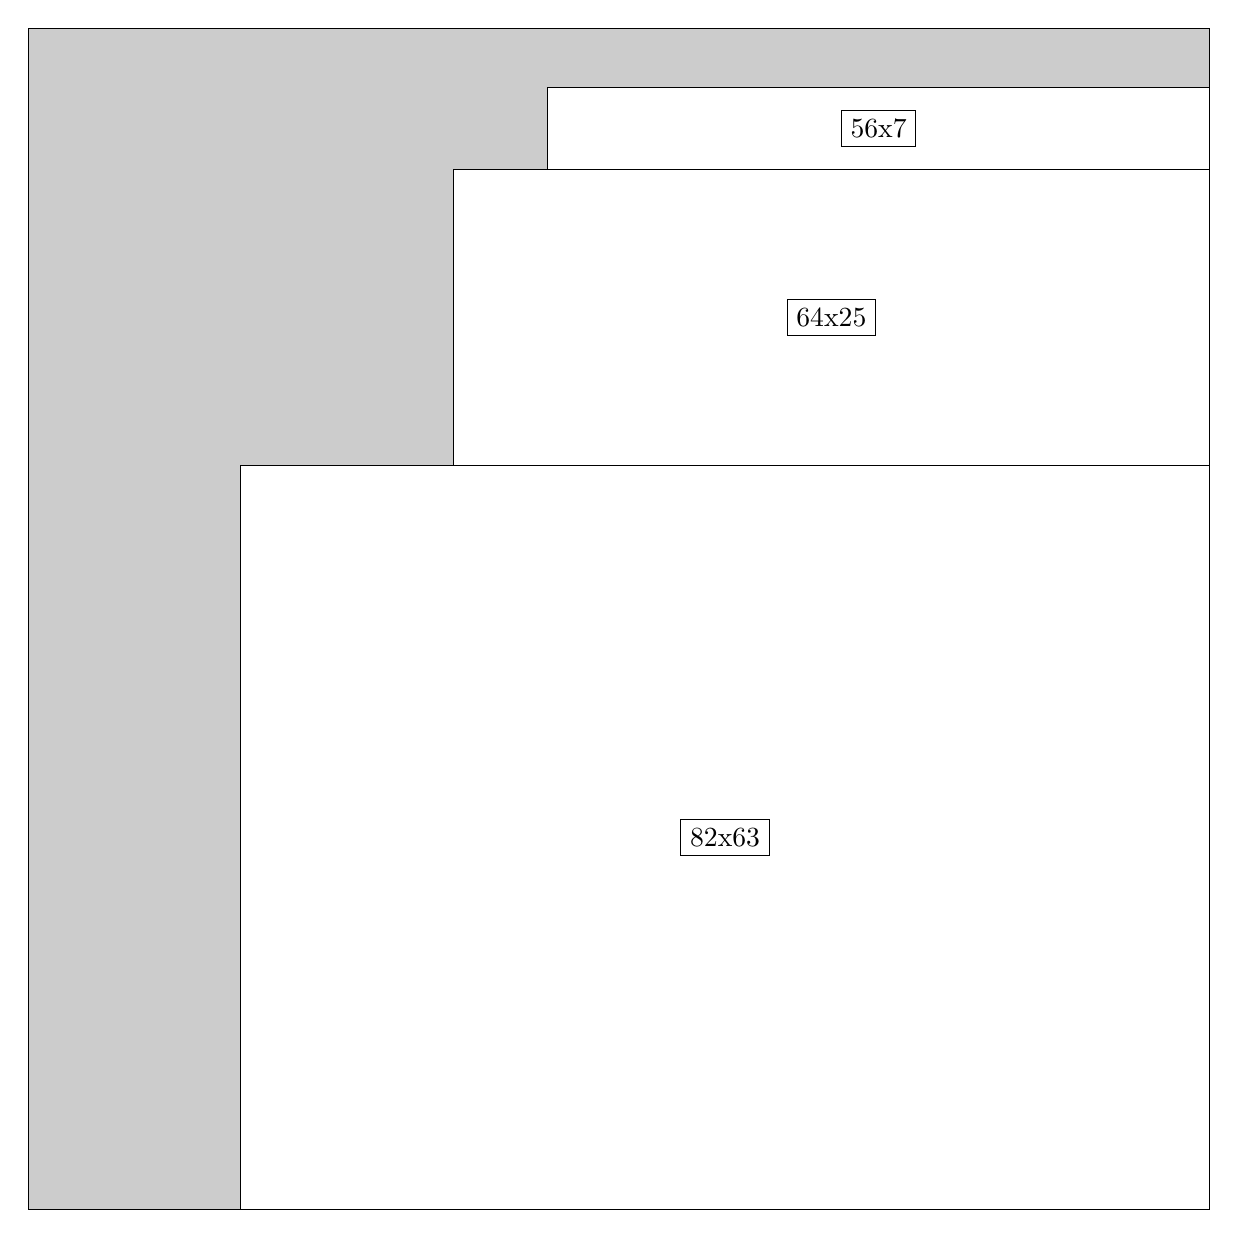
\begin{tikzpicture}[shorten >=1pt,scale=1.0,every node/.style={scale=1.0},->]
\tikzstyle{vertex}=[circle,fill=black!25,minimum size=14pt,inner sep=0pt]
\filldraw[fill=gray!40!white, draw=black] (0,0) rectangle (15.0,15.0);
\foreach \name/\x/\y/\w/\h in {82x63/2.6999999999999997/0.0/12.299999999999999/9.45,64x25/5.3999999999999995/9.45/9.6/3.75,56x7/6.6/13.2/8.4/1.05}
\filldraw[fill=white!40!white, draw=black] (\x,\y) rectangle node[draw] (\name) {\name} ++(\w,\h);
\end{tikzpicture}


w =82 , h =63 , x =18 , y =0 , v =5166
\par
w =64 , h =25 , x =36 , y =63 , v =1600
\par
w =56 , h =7 , x =44 , y =88 , v =392
\par
\newpage


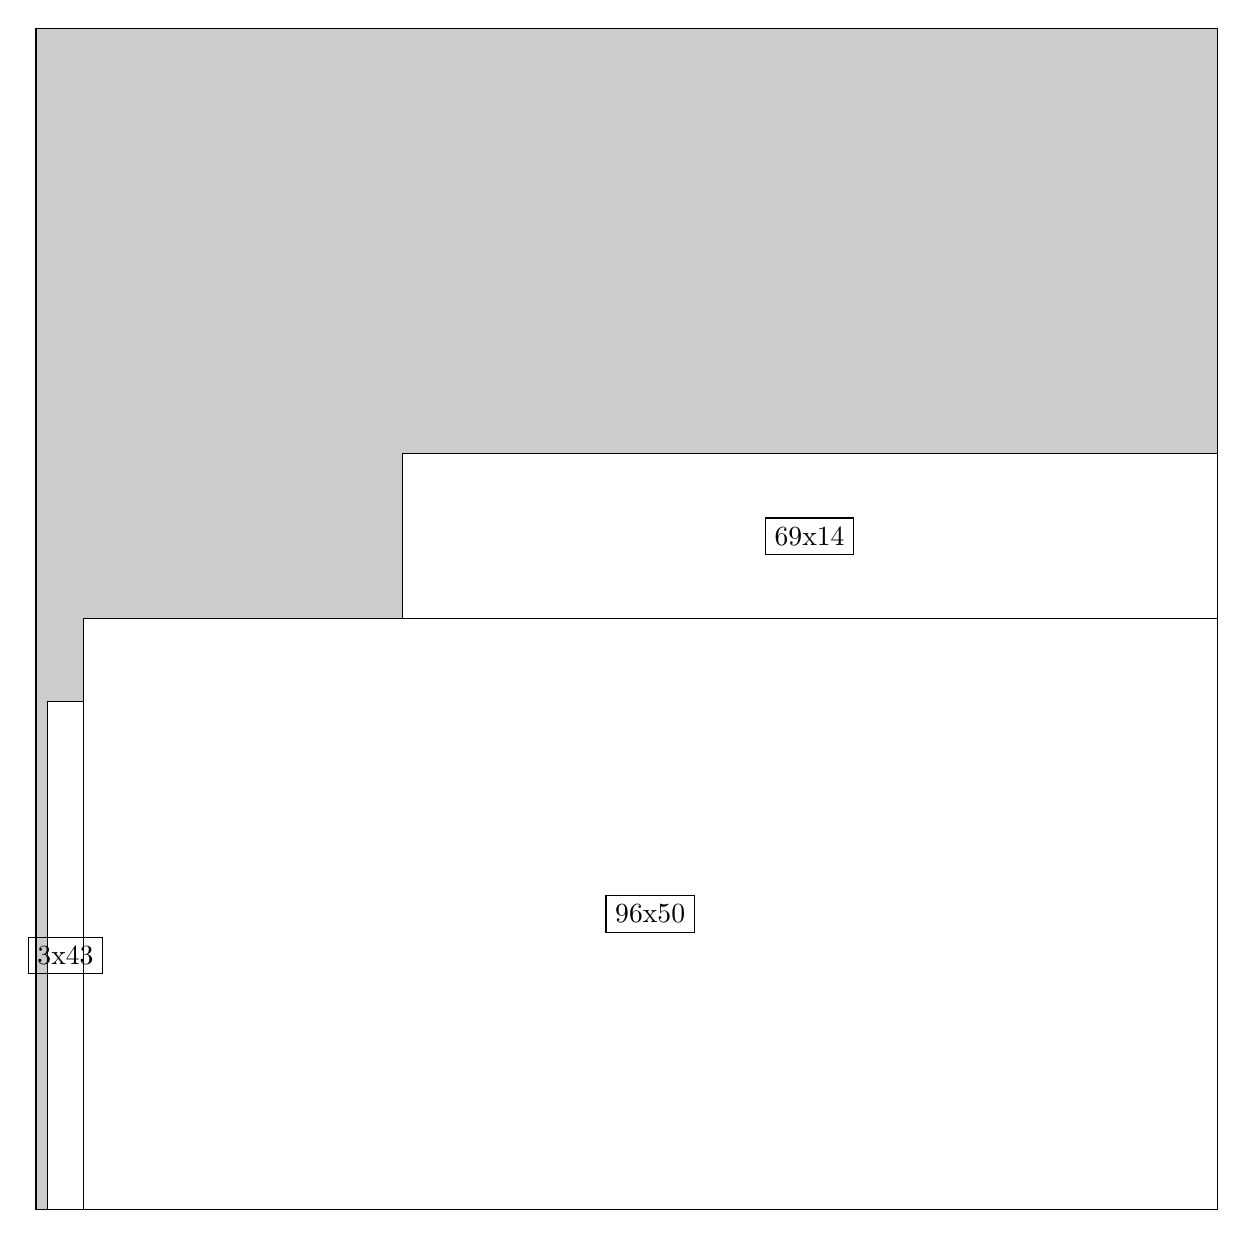
\begin{tikzpicture}[shorten >=1pt,scale=1.0,every node/.style={scale=1.0},->]
\tikzstyle{vertex}=[circle,fill=black!25,minimum size=14pt,inner sep=0pt]
\filldraw[fill=gray!40!white, draw=black] (0,0) rectangle (15.0,15.0);
\foreach \name/\x/\y/\w/\h in {96x50/0.6/0.0/14.399999999999999/7.5,3x43/0.15/0.0/0.44999999999999996/6.45,69x14/4.6499999999999995/7.5/10.35/2.1}
\filldraw[fill=white!40!white, draw=black] (\x,\y) rectangle node[draw] (\name) {\name} ++(\w,\h);
\end{tikzpicture}


w =96 , h =50 , x =4 , y =0 , v =4800
\par
w =3 , h =43 , x =1 , y =0 , v =129
\par
w =69 , h =14 , x =31 , y =50 , v =966
\par
\newpage


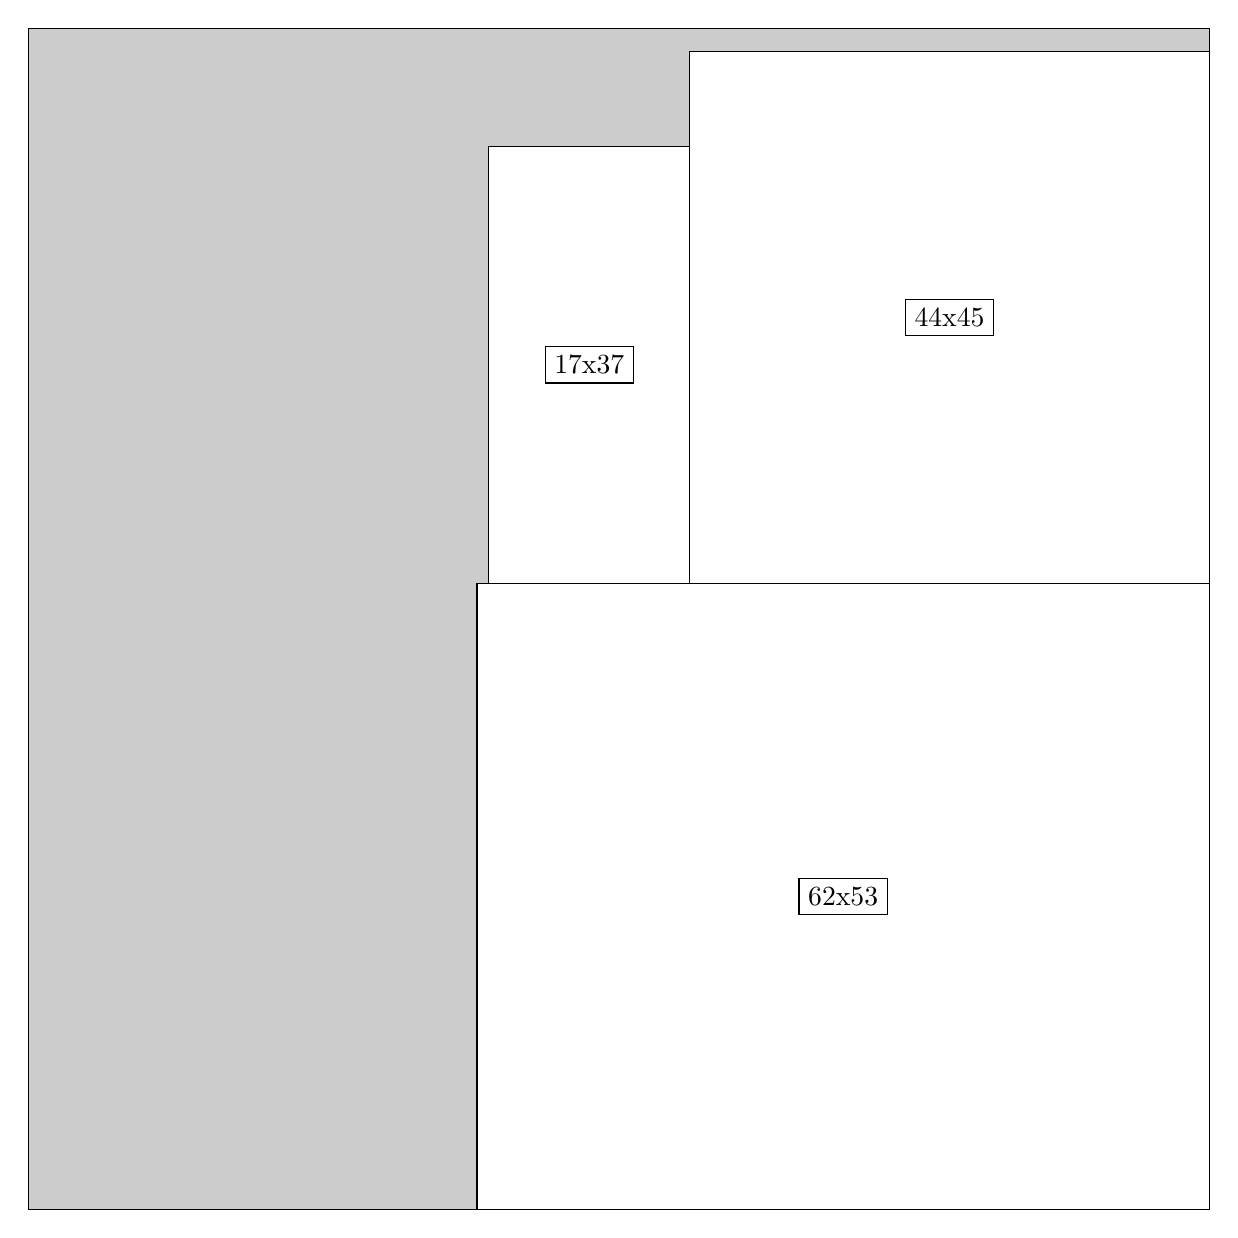
\begin{tikzpicture}[shorten >=1pt,scale=1.0,every node/.style={scale=1.0},->]
\tikzstyle{vertex}=[circle,fill=black!25,minimum size=14pt,inner sep=0pt]
\filldraw[fill=gray!40!white, draw=black] (0,0) rectangle (15.0,15.0);
\foreach \name/\x/\y/\w/\h in {62x53/5.7/0.0/9.299999999999999/7.949999999999999,44x45/8.4/7.949999999999999/6.6/6.75,17x37/5.85/7.949999999999999/2.55/5.55}
\filldraw[fill=white!40!white, draw=black] (\x,\y) rectangle node[draw] (\name) {\name} ++(\w,\h);
\end{tikzpicture}


w =62 , h =53 , x =38 , y =0 , v =3286
\par
w =44 , h =45 , x =56 , y =53 , v =1980
\par
w =17 , h =37 , x =39 , y =53 , v =629
\par
\newpage


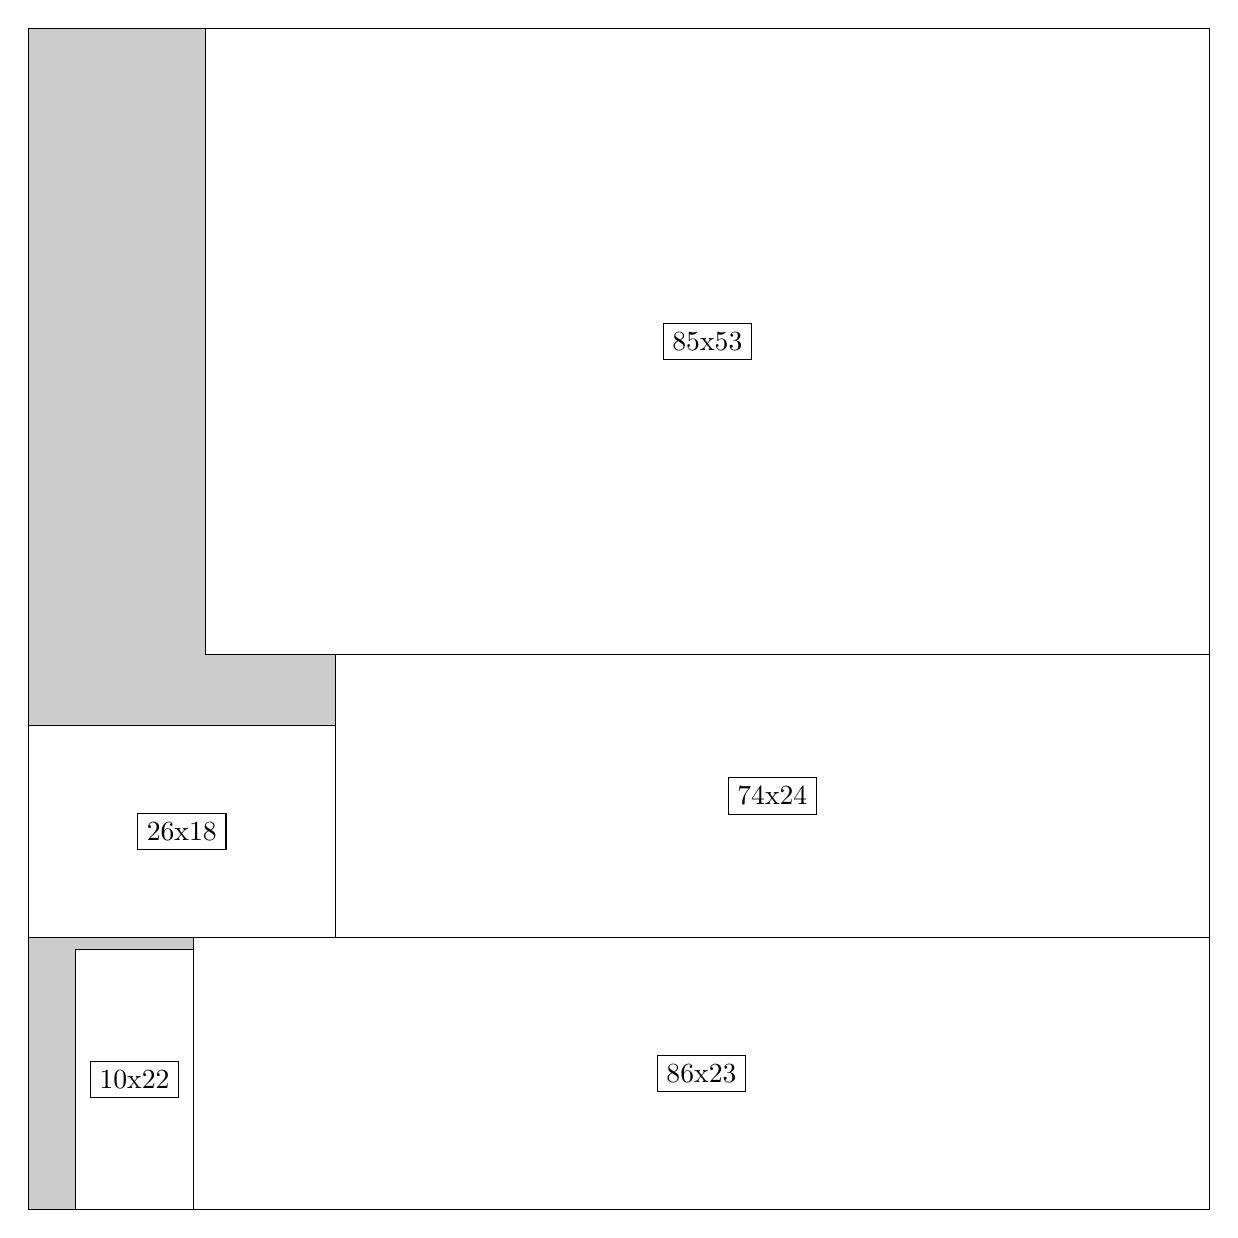
\begin{tikzpicture}[shorten >=1pt,scale=1.0,every node/.style={scale=1.0},->]
\tikzstyle{vertex}=[circle,fill=black!25,minimum size=14pt,inner sep=0pt]
\filldraw[fill=gray!40!white, draw=black] (0,0) rectangle (15.0,15.0);
\foreach \name/\x/\y/\w/\h in {86x23/2.1/0.0/12.9/3.4499999999999997,10x22/0.6/0.0/1.5/3.3,74x24/3.9/3.4499999999999997/11.1/3.5999999999999996,26x18/0.0/3.4499999999999997/3.9/2.6999999999999997,85x53/2.25/7.05/12.75/7.949999999999999}
\filldraw[fill=white!40!white, draw=black] (\x,\y) rectangle node[draw] (\name) {\name} ++(\w,\h);
\end{tikzpicture}


w =86 , h =23 , x =14 , y =0 , v =1978
\par
w =10 , h =22 , x =4 , y =0 , v =220
\par
w =74 , h =24 , x =26 , y =23 , v =1776
\par
w =26 , h =18 , x =0 , y =23 , v =468
\par
w =85 , h =53 , x =15 , y =47 , v =4505
\par
\newpage


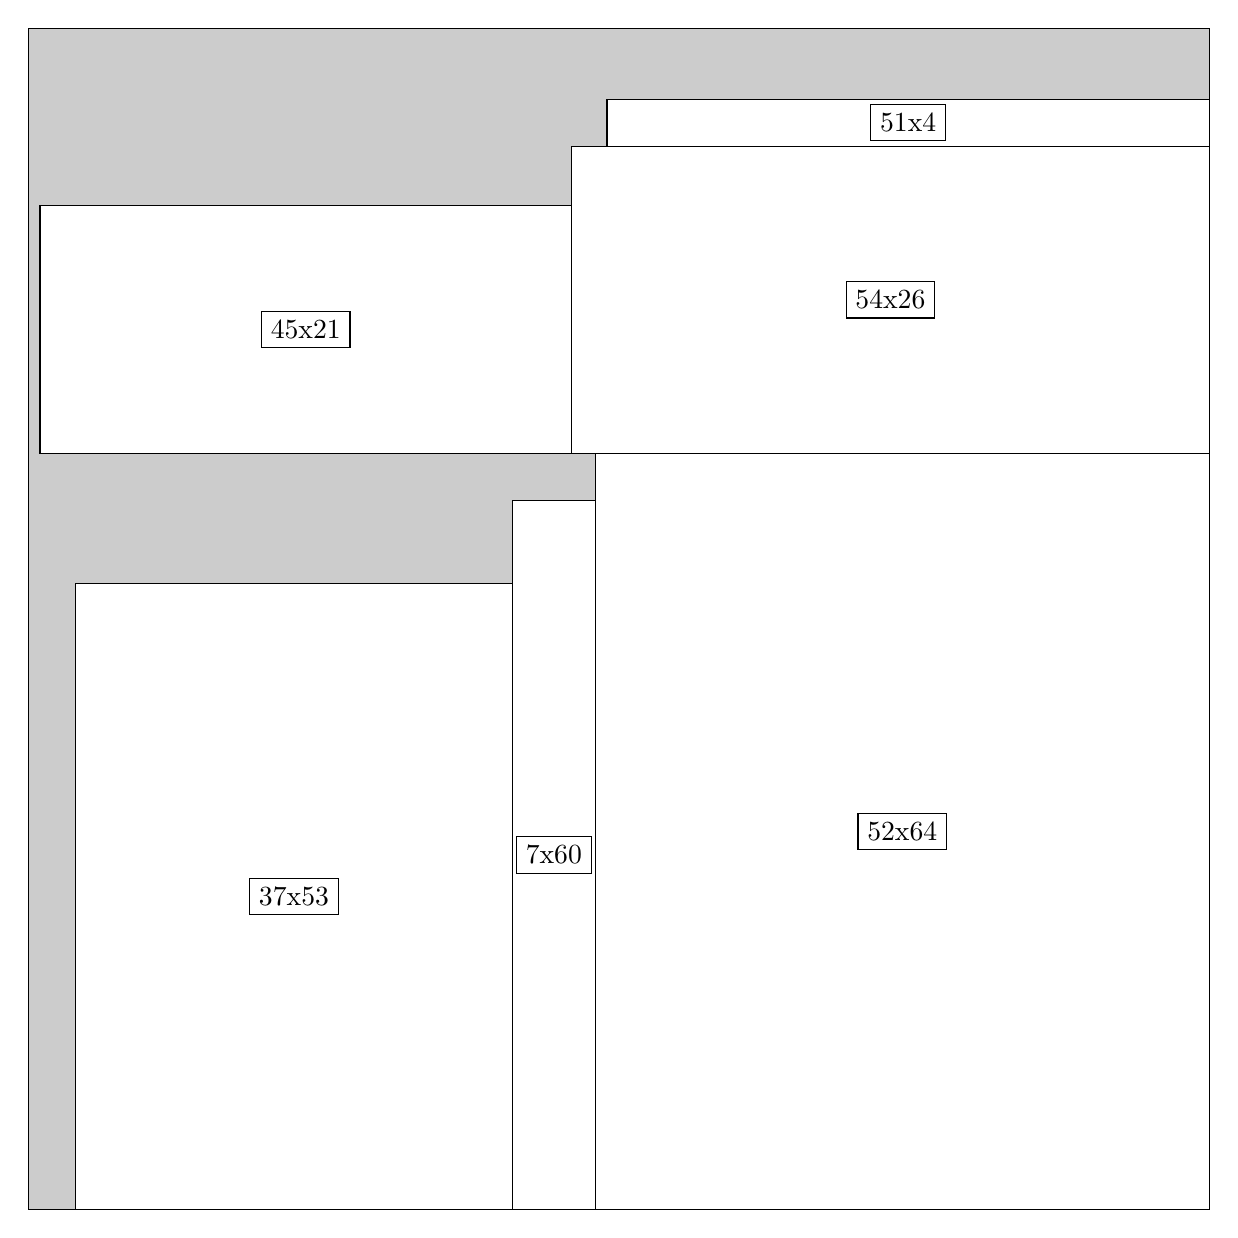
\begin{tikzpicture}[shorten >=1pt,scale=1.0,every node/.style={scale=1.0},->]
\tikzstyle{vertex}=[circle,fill=black!25,minimum size=14pt,inner sep=0pt]
\filldraw[fill=gray!40!white, draw=black] (0,0) rectangle (15.0,15.0);
\foreach \name/\x/\y/\w/\h in {52x64/7.199999999999999/0.0/7.8/9.6,7x60/6.1499999999999995/0.0/1.05/9.0,37x53/0.6/0.0/5.55/7.949999999999999,54x26/6.8999999999999995/9.6/8.1/3.9,51x4/7.35/13.5/7.6499999999999995/0.6,45x21/0.15/9.6/6.75/3.15}
\filldraw[fill=white!40!white, draw=black] (\x,\y) rectangle node[draw] (\name) {\name} ++(\w,\h);
\end{tikzpicture}


w =52 , h =64 , x =48 , y =0 , v =3328
\par
w =7 , h =60 , x =41 , y =0 , v =420
\par
w =37 , h =53 , x =4 , y =0 , v =1961
\par
w =54 , h =26 , x =46 , y =64 , v =1404
\par
w =51 , h =4 , x =49 , y =90 , v =204
\par
w =45 , h =21 , x =1 , y =64 , v =945
\par
\newpage


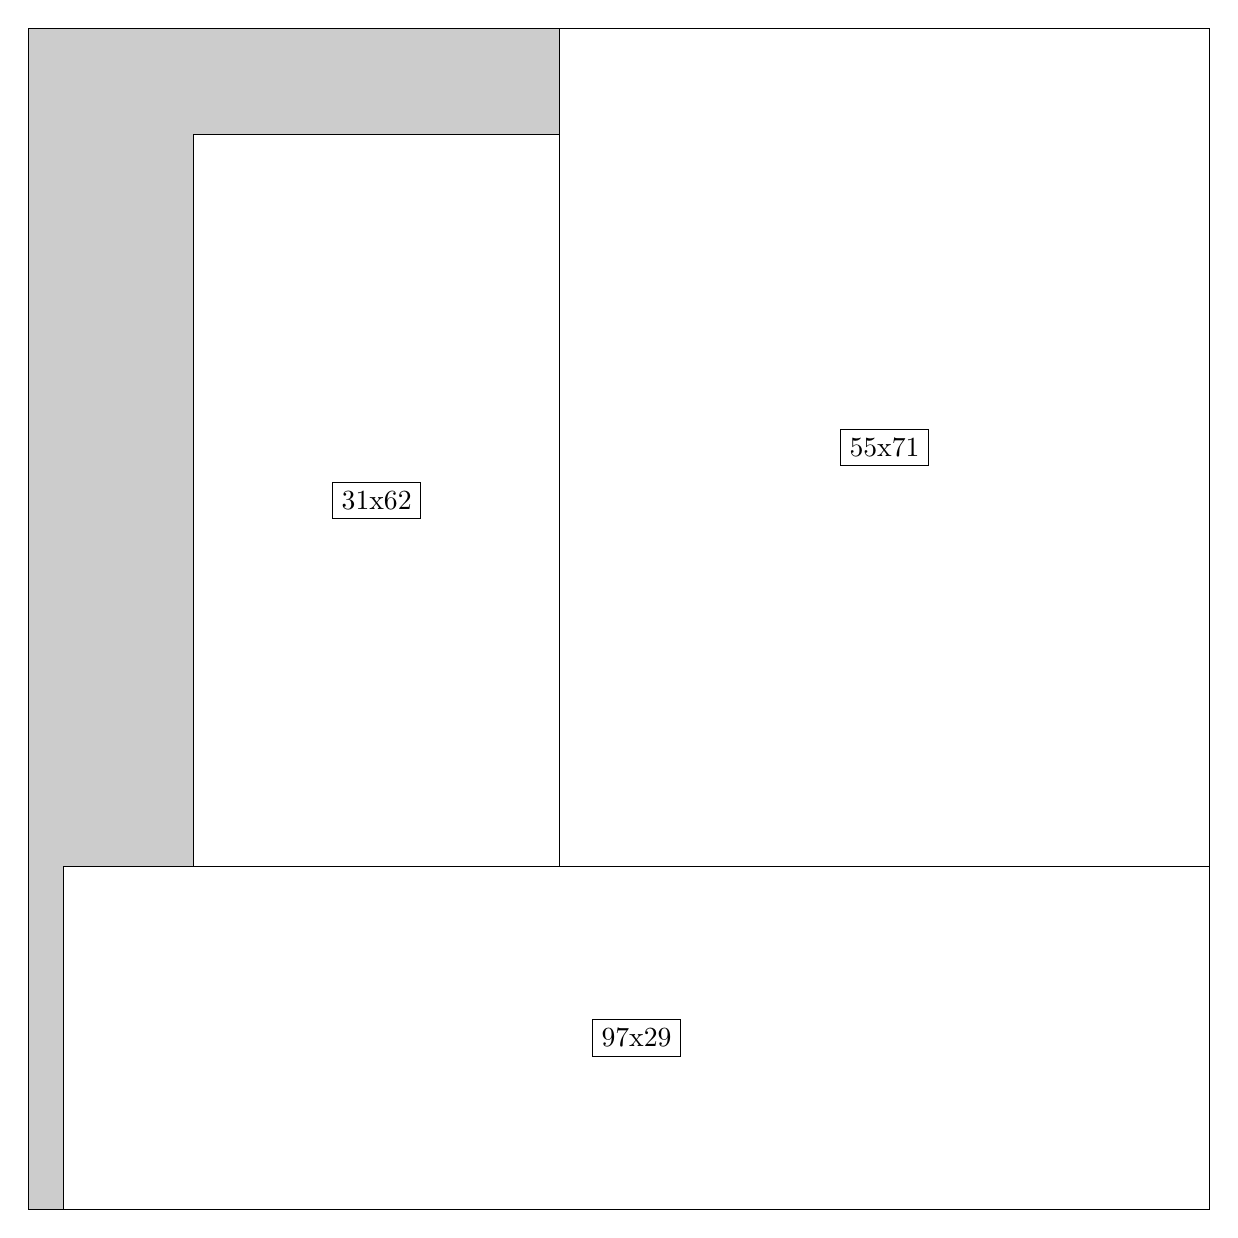
\begin{tikzpicture}[shorten >=1pt,scale=1.0,every node/.style={scale=1.0},->]
\tikzstyle{vertex}=[circle,fill=black!25,minimum size=14pt,inner sep=0pt]
\filldraw[fill=gray!40!white, draw=black] (0,0) rectangle (15.0,15.0);
\foreach \name/\x/\y/\w/\h in {97x29/0.44999999999999996/0.0/14.549999999999999/4.35,55x71/6.75/4.35/8.25/10.65,31x62/2.1/4.35/4.6499999999999995/9.299999999999999}
\filldraw[fill=white!40!white, draw=black] (\x,\y) rectangle node[draw] (\name) {\name} ++(\w,\h);
\end{tikzpicture}


w =97 , h =29 , x =3 , y =0 , v =2813
\par
w =55 , h =71 , x =45 , y =29 , v =3905
\par
w =31 , h =62 , x =14 , y =29 , v =1922
\par
\newpage


\end{document}